\chapter{Chapter Three}

\section{Event Comparisons}
Now, we consider each of the selected events individually, demonstrating that the events were classified correctly, and breaking down the results from each case. Although it is nearly impossible to extricate lake influence from synoptically classified events, synoptic-scale ascent is considered the characterizing factor. Descriptions of the synoptic pattern during each event are given without reference; For reference, see Appendix A for the 500mb Geopotential Heights, Skew-T charts, and Sounding Climatology utilized. These descriptions are ancillary to the study and are provided to demonstrate a variety of patterns are represented.

\begin{figure}[p]
\includegraphics[width=\textwidth]{grid/ref/20140118}
\caption{Gridded $Z_{eH}$ comparison for 18 January 2014. Time-average of all admitted scans.} 
\label{fig:grid_ref_20140118}
\end{figure}

\begin{figure}[p]
\includegraphics[width=\textwidth]{grid/zdr/20140118}
\caption{Gridded $Z_{DR}$ comparison for 18 January 2014. Time-average of all admitted scans.} 
\label{fig:grid_zdr_20140118}
\end{figure}

\begin{figure}[p]
\centering
   \begin{subfigure}{0.49\linewidth} \centering
     \includegraphics[scale=0.38]{scatter/ref/20140118}
     \caption{$Z_{eH}$ (dBZ)}\label{fig:scatter_ref_20140118}
   \end{subfigure}
   \begin{subfigure}{0.49\linewidth} \centering
     \includegraphics[scale=0.38]{scatter/zdr/20140118}
     \caption{$Z_{DR}$ (dB)}\label{fig:scatter_zdr_20140118}
   \end{subfigure}
\caption{Direct comparisons for 18 January 2014. Dataset includes all admitted grid cells.} \label{fig:scatter_20140118}
\end{figure}

\begin{figure}[p]
\includegraphics[width=0.75\textwidth]{hist/20140118}\centering
\caption{Histograms of $Z_{DR}$ (left), $Z_{DR}$ bias at CWKR, determined by subtracting the gridded, bias adjusted $Z_{DR}$ at KBUF from the $Z_{DR}$ at
CWKR. Both datasets exclude matched points with KDE $< 2$. } 
\label{fig:hist_20140118}
\end{figure}

\subsection{18 January 2014 - Synoptic}
In this event, a weak shortwave is approaching Southern Ontario as it rounds the base of a longwave trough centered over the Eastern seaboard of the US. 
Ample synoptic scale lift and a moist column through 500mb leads to scattered snow showers ahead of the shortwave. Figure \ref{fig:grid_ref_20140118} depicts
similiar cellular patterns between radars in the time-averaged $Z_{eH}$ field. In contrast, the $Z_{DR}$ comparison in Figure \ref{fig:grid_zdr_20140118}
shows that although the fields are similiar in their anisotropy, the spatial matching between the two is tenuous everywhere but in the heaviest showers. To
investigate further, we examine a scatter-plot directly comparing matched values between radars. Artifacts are present in both moments in Figure
\ref{fig:scatter_20140118}, indicated by evenly spaced vertical lines; these indicate an anomaly originating from the axis of which they are normal to. For
$Z_{eH}$, the artifacts are no longer present for values greater than 15 dBZ, which indicates that a stronger weather signal leads to better matching. In $Z_{DR}$ the artifacts are present throughout, but it is still possible to extract a signal from the noise. Data points with a normalized kernel density
greater than two are selected for the determination of bias between radars. Figure \ref{fig:hist_20140118} gives an estimate of the bias at CWKR, with a
value of -0.095 dB. This indicates that no discernible bias exists within the
error limit of $\pm$0.1 dB  during this event.


\begin{figure}[p]
\includegraphics[width=0.75\textwidth]{grid/ref/20140123}
\caption{Gridded $Z_{eH}$ comparison for 23 January 2014. Time-average of all admitted scans.} 
\label{fig:grid_ref_20140123}
\end{figure}

\begin{figure}[p]
\includegraphics[width=\textwidth]{grid/zdr/20140123}
\caption{Gridded $Z_{DR}$ comparison for 23 January 2014. Time-average of all admitted scans.} 
\label{fig:grid_zdr_20140123}
\end{figure}

\begin{figure}[p]
\centering
   \begin{subfigure}{0.49\linewidth} \centering
     \includegraphics[scale=0.38]{scatter/ref/20140123}
     \caption{$Z_{eH}$ (dBZ)}\label{fig:scatter_ref_20140123}
   \end{subfigure}
   \begin{subfigure}{0.49\linewidth} \centering
     \includegraphics[scale=0.38]{scatter/zdr/20140123}
     \caption{$Z_{DR}$ (dB)}\label{fig:scatter_zdr_20140123}
   \end{subfigure}
\caption{Direct comparisons for 23 January 2014. Dataset includes all admitted grid cells.} \label{fig:scatter_20140123}
\end{figure}

\begin{figure}[p]
\includegraphics[width=0.75\textwidth]{hist/20140123}\centering
\caption{Histograms of $Z_{DR}$ (left), $Z_{DR}$ bias at CWKR, determined by subtracting the gridded, bias adjusted $Z_{DR}$ at KBUF from the $Z_{DR}$ at CWKR. Both datasets exclude matched points with KDE $< 2$. } 
\label{fig:hist_20140123}
\end{figure}

\subsection{23 January 2014 - Lake-Effect}

A positively tilted longwave trough dominates the eastern third of Canada during this event, with NW winds at 850mb and SW winds at the surface. This light yet convergent flow yields the single, heavy band depicted in Figure \ref{fig:grid_ref_20140123}, colloquially referred to as ``tea-kettle'' lake-effect snow. There is also a background stream of very light lake-effect snow impinging from Lake Erie. Spatial banding patterns of the lake-effect snow in the time-averaged $Z_{eH}$ fields as compared between the radars are remarkably similar. In contrast, the $Z_{DR}$ comparison indicates that although the fields are similiar in their anisotropy, the spatial matching between the two is tenuous everywhere but in the heaviest showers.  An anistropic pattern is imparted on the $Z_{DR}$ fields by the light snow from Lake Erie, evident in Figure \ref{fig:grid_zdr_20140123}. The scatter-plot in Figure \ref{scatter_ref_20140123} shows a good fit for $Z_{eH}$ between radars, with the slope of the orthonormal  a is still possible to extract a signal from the noise. Data points with a normalized kernel density greater than two are selected for the determination of bias between radars. Figure \ref{fig:hist_20140123} gives an estimate of the bias at CWKR, with a value of -0.055 dB. Once again, no discernible bias exists within the error limit of $\pm$0.1 dB for this event.



\begin{figure}[p]
\includegraphics[width=\textwidth]{grid/ref/20140201}
\caption{Gridded $Z_{eH}$ comparison for 1 February 2014. Time-average of all admitted scans.} 
\label{fig:grid_ref_20140201}
\end{figure}

\begin{figure}[p]
\includegraphics[width=\textwidth]{grid/zdr/20140201}
\caption{Gridded $Z_{DR}$ comparison for 1 February 2014. Time-average of all admitted scans.} 
\label{fig:grid_zdr_20140201}
\end{figure}

\begin{figure}[p]
\centering
   \begin{subfigure}{0.49\linewidth} \centering
     \includegraphics[scale=0.38]{scatter/ref/20140201}
     \caption{$Z_{eH}$ (dBZ)}\label{fig:scatter_ref_20140201}
   \end{subfigure}
   \begin{subfigure}{0.49\linewidth} \centering
     \includegraphics[scale=0.38]{scatter/zdr/20140201}
     \caption{$Z_{DR}$ (dB)}\label{fig:scatter_zdr_20140201}
   \end{subfigure}
\caption{Direct comparisons for 1 February 2014. Dataset includes all admitted grid cells.} \label{fig:scatter_20140201}
\end{figure}

\begin{figure}[p]
\includegraphics[width=0.75\textwidth]{hist/20140201}\centering
\caption{Histograms of $Z_{DR}$ (left), $Z_{DR}$ bias at CWKR, determined by subtracting the gridded, bias adjusted $Z_{DR}$ at KBUF from the $Z_{DR}$ at CWKR. Both datasets exclude matched points with KDE $< 2$. } 
\label{fig:hist_20140201}
\end{figure}

\subsection{1 February 2014 - Synoptic}
This event is characterized by strong SW flow aloft, with above average moisture content. This leads to widespread stratiform snow, with an eventual transition to rain outside of the time interval selected.  

\begin{figure}[p]
\includegraphics[width=\textwidth]{grid/ref/20150106}
\caption{Gridded $Z_{eH}$ comparison for 6 January 2015. Time-average of all admitted scans.} 
\label{fig:grid_ref_20150106}
\end{figure}

\begin{figure}[p]
\includegraphics[width=\textwidth]{grid/zdr/20150106}
\caption{Gridded $Z_{DR}$ comparison for 6 January 2015. Time-average of all admitted scans.} 
\label{fig:grid_zdr_20150106}
\end{figure}

\begin{figure}[p]
\centering
   \begin{subfigure}{0.49\linewidth} \centering
     \includegraphics[scale=0.38]{scatter/ref/20150106}
     \caption{$Z_{eH}$ (dBZ)}\label{fig:scatter_ref_20150106}
   \end{subfigure}
   \begin{subfigure}{0.49\linewidth} \centering
     \includegraphics[scale=0.38]{scatter/zdr/20150106}
     \caption{$Z_{DR}$ (dB)}\label{fig:scatter_zdr_20150106}
   \end{subfigure}
\caption{Direct comparisons for 6 January 2015. Dataset includes all admitted grid cells.} \label{fig:scatter_20150106}
\end{figure}

\begin{figure}[p]
\includegraphics[width=0.75\textwidth]{hist/20150106}\centering
\caption{Histograms of $Z_{DR}$ (left), $Z_{DR}$ bias at CWKR, determined by subtracting the gridded, bias adjusted $Z_{DR}$ at KBUF from the $Z_{DR}$ at CWKR. Both datasets exclude matched points with KDE $< 2$. } 
\label{fig:hist_20150106}
\end{figure}

\subsection{6 January 2015 - Lake-Effect}
A highly zonal, NW flow aloft is present in this case, typical of lake-effect snow for the Great Lakes region. Anemic in radar appearance, a lake-effect band develops in the light winds near the surface; this case could be characterized as a weak ``tea-kettle'' event. Figure \ref{fig:grid_ref_20150106} depicts the time-averaged $Z_{eH}$ during the event.
\begin{figure}[p]
\includegraphics[width=\textwidth]{grid/ref/20150107}
\caption{Gridded $Z_{eH}$ comparison for 7 January 2015. Time-average of all admitted scans.} 
\label{fig:grid_ref_20150107}
\end{figure}

\begin{figure}[p]
\includegraphics[width=\textwidth]{grid/zdr/20150107}
\caption{Gridded $Z_{DR}$ comparison for 7 January 2015. Time-average of all admitted scans.} 
\label{fig:grid_zdr_20150107}
\end{figure}

\begin{figure}[p]
\centering
   \begin{subfigure}{0.49\linewidth} \centering
     \includegraphics[scale=0.38]{scatter/ref/20150107}
     \caption{$Z_{eH}$ (dBZ)}\label{fig:scatter_ref_20150107}
   \end{subfigure}
   \begin{subfigure}{0.49\linewidth} \centering
     \includegraphics[scale=0.38]{scatter/zdr/20150107}
     \caption{$Z_{DR}$ (dB)}\label{fig:scatter_zdr_20150107}
   \end{subfigure}
\caption{Direct comparisons for 7 January 2015. Dataset includes all admitted grid cells.} \label{fig:scatter_20150107}
\end{figure}

\begin{figure}[p]
\includegraphics[width=0.75\textwidth]{hist/20150107}\centering
\caption{Histograms of $Z_{DR}$ (left), $Z_{DR}$ bias at CWKR, determined by subtracting the gridded, bias adjusted $Z_{DR}$ at KBUF from the $Z_{DR}$ at CWKR. Both datasets exclude matched points with KDE $< 2$. } 
\label{fig:hist_20150107}
\end{figure}

\subsection{7 January 2015 - Synoptic}
Less than 24 hours after the previous event, the zonal flow has buckled and a strong shortwave is approaching Southern Ontario. Radar animations indicate a cold front passage over the lake occurs.
Figure \ref{fig:grid_ref_20150107} shows a solid band of snow progressed from mid-lake southward.
\begin{figure}[p]
\includegraphics[width=\textwidth]{grid/ref/20150206}
\caption{Gridded $Z_{eH}$ comparison for 6 February 2015. Time-average of all admitted scans.} 
\label{fig:grid_ref_20150206}
\end{figure}

\begin{figure}[p]
\includegraphics[width=\textwidth]{grid/zdr/20150206}
\caption{Gridded $Z_{DR}$ comparison for 6 February 2015. Time-average of all admitted scans.} 
\label{fig:grid_zdr_20150206}
\end{figure}

\begin{figure}[p]
\centering
   \begin{subfigure}{0.49\linewidth} \centering
     \includegraphics[scale=0.38]{scatter/ref/20150206}
     \caption{$Z_{eH}$ (dBZ)}\label{fig:scatter_ref_20150206}
   \end{subfigure}
   \begin{subfigure}{0.49\linewidth} \centering
     \includegraphics[scale=0.38]{scatter/zdr/20150206}
     \caption{$Z_{DR}$ (dB)}\label{fig:scatter_zdr_20150206}
   \end{subfigure}
\caption{Direct comparisons for 6 February 2015. Dataset includes all admitted grid cells.} \label{fig:scatter_20150206}
\end{figure}

\begin{figure}[p]
\includegraphics[width=0.75\textwidth]{hist/20150206}\centering
\caption{Histograms of $Z_{DR}$ (left), $Z_{DR}$ bias at CWKR, determined by subtracting the gridded, bias adjusted $Z_{DR}$ at KBUF from the $Z_{DR}$ at CWKR. Both datasets exclude matched points with KDE $< 2$. } 
\label{fig:hist_20150206}
\end{figure}


\subsection{6 February 2015 - Synoptic}
For this event, Southern Ontario is on the backside of shortwave, with a frontal passage occuring once again.
\begin{figure}[p]
\includegraphics[width=\textwidth]{grid/ref/20150214}
\caption{Gridded $Z_{eH}$ comparison for 14 February 2015. Time-average of all admitted scans.} 
\label{fig:grid_ref_20150214}
\end{figure}

\begin{figure}[p]
\includegraphics[width=\textwidth]{grid/zdr/20150214}
\caption{Gridded $Z_{DR}$ comparison for 14 February 2015. Time-average of all admitted scans.} 
\label{fig:grid_zdr_20150214}
\end{figure}

\begin{figure}[p]
\centering
   \begin{subfigure}{0.49\linewidth} \centering
     \includegraphics[scale=0.38]{scatter/ref/20150214}
     \caption{$Z_{eH}$ (dBZ)}\label{fig:scatter_ref_20150214}
   \end{subfigure}
   \begin{subfigure}{0.49\linewidth} \centering
     \includegraphics[scale=0.38]{scatter/zdr/20150214}
     \caption{$Z_{DR}$ (dB)}\label{fig:scatter_zdr_20150214}
   \end{subfigure}
\caption{Direct comparisons for 14 February 2015. Dataset includes all admitted grid cells.} \label{fig:scatter_20150214}
\end{figure}

\begin{figure}[p]
\includegraphics[width=0.75\textwidth]{hist/20150214}\centering
\caption{Histograms of $Z_{DR}$ (left), $Z_{DR}$ bias at CWKR, determined by subtracting the gridded, bias adjusted $Z_{DR}$ at KBUF from the $Z_{DR}$ at CWKR. Both datasets exclude matched points with KDE $< 2$. } 
\label{fig:hist_20150214}
\end{figure}


\subsection{14 February 2015 - Lake-Effect}
While Southern Ontario is bracing for the impact of a bowling-ball like lobe of the polar vortex, strong W to SW flow from the surface to 850mb allows for a prolonged period of lake-effect snow over the lake. 
\begin{figure}[p]
\includegraphics[width=\textwidth]{grid/ref/20150218}
\caption{Gridded $Z_{eH}$ comparison for 18 February 2015. Time-average of all admitted scans.} 
\label{fig:grid_ref_20150218}
\end{figure}

\begin{figure}[p]
\includegraphics[width=\textwidth]{grid/zdr/20150218}
\caption{Gridded $Z_{DR}$ comparison for 18 February 2015. Time-average of all admitted scans.} 
\label{fig:grid_zdr_20150218}
\end{figure}

\begin{figure}[p]
\centering
   \begin{subfigure}{0.49\linewidth} \centering
     \includegraphics[scale=0.38]{scatter/ref/20150218}
     \caption{$Z_{eH}$ (dBZ)}\label{fig:scatter_ref_20150218}
   \end{subfigure}
   \begin{subfigure}{0.49\linewidth} \centering
     \includegraphics[scale=0.38]{scatter/zdr/20150218}
     \caption{$Z_{DR}$ (dB)}\label{fig:scatter_zdr_20150218}
   \end{subfigure}
\caption{Direct comparisons for 18 February 2015. Dataset includes all admitted grid cells.} \label{fig:scatter_20150218}
\end{figure}

\begin{figure}[p]
\includegraphics[width=0.75\textwidth]{hist/20150218}\centering
\caption{Histograms of $Z_{DR}$ (left), $Z_{DR}$ bias at CWKR, determined by subtracting the gridded, bias adjusted $Z_{DR}$ at KBUF from the $Z_{DR}$ at CWKR. Both datasets exclude matched points with KDE $< 2$. } 
\label{fig:hist_20150218}
\end{figure}

\subsection{18 February 2015 - Lake-Effect}
Four days later, The polar vortex has arrived in earnest for this event, with the 500 dm isoheight nearing as far south as Windsor, ON. The cold airmass allows for the development of an intense lake-effect snow band, the strongest of all the lake-effect cases as indicated by the $Z_{eH}$ means in Figure \ref{fig:grid_ref_20150218}. 
\begin{figure}[p]
\includegraphics[width=\textwidth]{grid/ref/20160210}
\caption{Gridded $Z_{eH}$ comparison for 10 February 2016. Time-average of all admitted scans.} 
\label{fig:grid_ref_20160210}
\end{figure}

\begin{figure}[p]
\includegraphics[width=\textwidth]{grid/zdr/20160210}
\caption{Gridded $Z_{DR}$ comparison for 10 February 2016. Time-average of all admitted scans.} 
\label{fig:grid_zdr_20160210}
\end{figure}

\begin{figure}[p]
\centering
   \begin{subfigure}{0.49\linewidth} \centering
     \includegraphics[scale=0.38]{scatter/ref/20160210}
     \caption{$Z_{eH}$ (dBZ)}\label{fig:scatter_ref_20160210}
   \end{subfigure}
   \begin{subfigure}{0.49\linewidth} \centering
     \includegraphics[scale=0.38]{scatter/zdr/20160210}
     \caption{$Z_{DR}$ (dB)}\label{fig:scatter_zdr_20160210}
   \end{subfigure}
\caption{Direct comparisons for 10 February 2016. Dataset includes all admitted grid cells.} \label{fig:scatter_20160210}
\end{figure}

\begin{figure}[p]
\includegraphics[width=0.75\textwidth]{hist/20160210}\centering
\caption{Histograms of $Z_{DR}$ (left), $Z_{DR}$ bias at CWKR, determined by subtracting the gridded, bias adjusted $Z_{DR}$ at KBUF from the $Z_{DR}$ at CWKR. Both datasets exclude matched points with KDE $< 2$. } 
\label{fig:hist_20160210}
\end{figure}

\subsection{10 February 2016 - Lake-Effect}
The 500mb ridge axis is centered to the south of Southern Ontario in the Appalachians, with WNW flow aloft during this event. With a slight amount of pre-existing instability augmenting the lake induced instabilities, a healthly band of convection forms on the southern end of the lake. 
non-existent directional shear from the surface to 850mb
\begin{figure}[p]
\includegraphics[width=\textwidth]{grid/ref/20161215}
\caption{Gridded $Z_{eH}$ comparison for 15 December 2016. Time-average of all admitted scans.} 
\label{fig:grid_ref_20161215}
\end{figure}

\begin{figure}[p]
\includegraphics[width=\textwidth]{grid/zdr/20161215}
\caption{Gridded $Z_{DR}$ comparison for 15 December 2016. Time-average of all admitted scans.} 
\label{fig:grid_zdr_20161215}
\end{figure}

\begin{figure}[p]
\centering
   \begin{subfigure}{0.49\linewidth} \centering
     \includegraphics[scale=0.38]{scatter/ref/20161215}
     \caption{$Z_{eH}$ (dBZ)}\label{fig:scatter_ref_20161215}
   \end{subfigure}
   \begin{subfigure}{0.49\linewidth} \centering
     \includegraphics[scale=0.38]{scatter/zdr/20161215}
     \caption{$Z_{DR}$ (dB)}\label{fig:scatter_zdr_20161215}
   \end{subfigure}
\caption{Direct comparisons for 15 December 2016. Dataset includes all admitted grid cells.} \label{fig:scatter_20161215}
\end{figure}

\begin{figure}[p]
\includegraphics[width=0.75\textwidth]{hist/20161215}\centering
\caption{Histograms of $Z_{DR}$ (left), $Z_{DR}$ bias at CWKR, determined by subtracting the gridded, bias adjusted $Z_{DR}$ at KBUF from the $Z_{DR}$ at CWKR. Both datasets exclude matched points with KDE $< 2$. } 
\label{fig:hist_20161215}
\end{figure}

\subsection{15 December 2016 - Synoptic}
A deep longwave trough is centered over Southern Ontario, within an Arctic airmass in place over the Great Lakes region. With meager moisture in place, a post-frontal trough manages to squeeze out some passing snow-showers, indicated in Figure \ref{fig:grid_ref_20161215}.


\begin{figure}[h]
\centering
   \begin{subfigure}{0.49\linewidth} \centering
     \includegraphics[scale=0.45]{ref_scatter_synoptic}
     \caption{subset of synoptic snow events}\label{fig:ref_synoptic}
   \end{subfigure}
   \begin{subfigure}{0.49\linewidth} \centering
     \includegraphics[scale=0.45]{ref_scatter_lake_effect}
     \caption{subset of lake-effect snow events}\label{fig:ref_lake_effect}
   \end{subfigure}
\caption{Scatter-plots of CWKR versus KBUF grid analyzed reflectivity, with Kernel Density Estimation shading. The red line is an Orthonormal Linear Regression, with a black identity line.} \label{fig:ref_scatter}
\end{figure}

\subsection{$Z_{eH}$ Subset Direct Comparisons}
The first direct comparisons are shown in Figure \ref{fig:ref_scatter}, with a scatter-plot of KBUF $Z_{eH}$ data versus CWKR on the common grid. Figure \ref{fig:ref_synoptic} is the subset of synoptic events while Figure \ref{fig:ref_lake_effect} is the subset of lake-effect events. These results show that lake-effect snow events achieve a better match between the radars than synoptic events; there is a sample size caveat due to synoptic subset only containing about a third of the matched points than those in in the synoptic subset. Another result shown in Figure \ref{fig:ref_scatter} is that CWKR is slightly under-reporting reflectivity in the 15-25 dBZ range for lake-effect events, while it over-reports for synoptic events. In order to examine this further, we turn to Figure \ref{fig:grid_ref}, revealing heavier banding closer to KBUF (south of $43.4^{\circ}$ N and east of $79^{\circ}$ W) in lake-effect events. Due to the bands location farther away from CWKR, its beam is most likely overshooting this shallow lake effect band. This is confirmed by the pattern in the reflectivity differences, which reveals a stronger range dependency in lake-effect events than synoptic. Another notable feature in Figure \ref{fig:grid_ref} is the resolution of finer scale features by CWKR is superior, especially for the lake-effect banding patterns around mid-lake. This is likely a function of its narrower physical beamwidth.

\begin{figure}
\includegraphics[width=\textwidth]{grid_ref.png}\vspace*{-5mm} 
\caption{Time averaged subsets of grid $Z_{eH}$ for KBUF and CWKR, with differences between the radars for each subset shown in the bottom panel.}
\label{fig:grid_ref}
\end{figure}

\begin{figure}[h]
\centering
   \begin{subfigure}{0.49\linewidth} \centering
     \includegraphics[scale=0.4]{zdr_scatter_synoptic.png}
     \caption{subset of synoptic snow events}\label{fig:zdr_scatter_synoptic}
   \end{subfigure}
   \begin{subfigure}{0.49\linewidth} \centering
     \includegraphics[scale=0.4]{zdr_scatter_lake_effect.png}
     \caption{subset of lake-effect snow events}\label{fig:zdr_scatter_lake_effect}
   \end{subfigure}
\caption{Scatter-plots of CWKR versus KBUF grid analyzed differential reflectivity, with Kernel Density Estimation shading. The red line is an Orthonormal Linear Regression, with a black identity line.} \label{fig:zdr_scatter}
\end{figure}

\begin{figure}
\includegraphics[width=\textwidth]{KBUF_bias_2014_jan-march.png}
\caption{Graphs of KBUF January-March 2014 $Z_{DR}$ bias estimates from NEXRAD rain (top panel) and snow (bottom panel) methods. Shading is a seven-day running median and points are daily median values. Tolerance levels are shaded light blue from $\pm0.2$ dB. It is shown here that KBUF is outside of calibration tolerances. Data collected from archived NEXRAD Level III data.} 
\label{fig:KBUF_bias_2014_jan-march}
\end{figure}





To investigate this further, we turn to a NEXRAD Level III algorithm which estimates $Z_{DR}$ biases using external targets, as discussed by \cite{Cunningham2013}. For the first lake-effect snow event on 23 January 2014, the $Z_{DR}$ bias estimate at KBUF from the rain and snow methods shown in Figure \ref{fig:KBUF_bias_2014_jan-march} is approximately -0.4 dB, as given by the seven-day running median. This compares well with the bias estimate made by comparing KBUF with CWKR with all hydrometeor classes admitted, shown in Figure \ref{fig:20140123hist_all}. When only dry snow bins are admitted though, the bias becomes masked, with Figure \ref{fig:20140123hist_ds} showing a bias of nearly 0 dB. Figure \ref{fig:KBUF_bias_2014_apr-june} gives an example of a period when the radar is fixed and comes back into calibration. In contrast, during a synpotic snowfall event on 9 February 2014, Figure ref{fig:20140209hist} shows that the dry snow filtering technique yields the best estimate of bias. 




\subsection{$Z_{DR}$ Subset Direct Comparison}
When comparing $Z_{DR}$ in the same manner as $Z_{eH}$, no clear pattern emerges. The analyzed values are highly uncorrelated, as shown in Figure \ref{fig:zdr_scatter}. Unlike reflectivity, differential reflectivity is a relative quantity, and is much more sensitive to biases. Therefore, each case will be considered individually to estimate an event bias, if any. The externally estimated $Z_{DR}$ bias from KBUF is subtracted out to give the bias at CWKR.


\section{Initial Results}
The main advantage of the common grid is that it allows for direct one-to-one comparison between the two radars. By directly interrogating the base moments, the veracity of the analysis technique is ensured, and any artifacts are identifiable. This will also help characterize differences between lake-effect and synoptic snow events, in terms of objective analyzability and performance of the radar systems in resolving snowfall at meso-$\beta$ length scales versus synpotic length scales. As these are direct comparisons of radar data, hereafter the terms under(over)-reporting will be used to describe an estimate one radar makes in comparison with the other.
